\documentclass[10pt,twocolumn]{article}
% NOTE: formatted with the generic article class because IEEEtran.cls is not installed in the authoring
% sandbox.  Swap to \documentclass[conference]{IEEEtran} (or the target venue template) before submission.
\usepackage[a4paper,margin=0.8in,columnsep=0.25in]{geometry}
\usepackage[T1]{fontenc}
\usepackage[expansion=false]{microtype}
\usepackage{booktabs,graphicx,amsmath,xcolor,enumitem,hyperref,array,multirow}
\usepackage[font=small,labelfont=bf]{caption}
\hypersetup{colorlinks=true,linkcolor=blue!50!black,urlcolor=blue!50!black,citecolor=blue!50!black}
\setlist{nosep,leftmargin=*}
% Visible marker for anything that must still be (re-)run on the author's data before submission.
\newcommand{\pending}[1]{\textcolor{red!70!black}{\textbf{[TO RUN: #1]}}}
\newcommand{\F}{F_1}

\title{\vspace{-1.0em}Event Duration, Alert Budgets and Metric Choice in Energy Time-Series Anomaly Detection: A Controlled Re-examination\vspace{-0.4em}}
\author{Sulman Younas\\ \small Independent researcher, Edinburgh, UK \quad \texttt{sulmanyounas93@gmail.com}}
\date{}

\begin{document}
\maketitle
\vspace{-1.2em}

\begin{abstract}
A four-dataset comparison of five anomaly detectors on energy data (commodity prices, a simulated European grid, GB and Texas demand) appeared to show that the ranking of density-based and sequence-based detectors inverts as events span more native-resolution samples, with a ``detection gap'' at intermediate scale. Re-examining that comparison under a single evaluation contract, we find that these conclusions were not supported: one headline F1 mixed event-level recall with timestamp-level precision (0.695 versus 0.344 on a consistent timestamp-level definition); a fixed 5\% alert budget caps F1 by anomaly prevalence; and DBSCAN's realised alert rate floats far from that budget. We then run a controlled sweep in which prevalence is held at 3\% while event duration (2\,h--14\,d) and sampling resolution (30\,min, 1\,h, 1\,d) vary independently, with two event types and ten seeds. The best detector depends on event duration relative to the detector's own time scale; changing resolution from 30\,min to 1\,h changes DBSCAN's F1 by at most 0.022; and thresholded F1 and threshold-free AUC-PR disagree sharply for some detectors. Real-data results are reported descriptively because each dataset has only one or two events. All code, tests and result files are released.
\end{abstract}

\section{Introduction}
Choosing an anomaly detector for energy time series is a practical problem, and published benchmarks rarely hold the pipeline fixed while the data regime changes. An earlier version of this work did so for five detectors on four datasets and concluded that (i) the ranking of density-based (DBSCAN) and sequence-reconstruction (LSTM autoencoder) detectors inverts with the number of native-resolution samples an event spans, (ii) this supports a selection rule, and (iii) a ``detection gap'' exists at intermediate scale. Review of that version identified problems in the evidence: mixed metrics, confounded variables, one or two events per dataset, unequal tuning, and missing related work. This paper reports what remains true after correcting them. We do \emph{not} propose a new detector; the contribution is empirical and methodological:
\begin{enumerate}
\item A single evaluation contract (Sec.~\ref{sec:protocol}) separating event-level from timestamp-level metrics, reporting prevalence, the F1 ceiling implied by the alert budget, and a threshold-free metric. We show quantitatively how departures from it changed earlier conclusions.
\item A constant-prevalence controlled sweep over event duration and sampling resolution (Sec.~\ref{sec:sweep}), with two event types and ten seeds, which separates variables that were confounded across datasets.
\item A descriptive re-evaluation of the real-data results (Sec.~\ref{sec:real}) with every number traceable to a result file, and an explicit list of claims withdrawn.
\item Released code with unit tests for the metric and windowing logic, including regression tests for two bugs found during this revision.
\end{enumerate}

\section{Related Work}
Several benchmark and evaluation studies are directly relevant. TSB-UAD~\cite{paparrizos2022tsb} collects 13{,}766 labelled univariate series and evaluates twelve detectors; TSB-AD~\cite{liu2024elephant} curates 40 datasets and 40 detectors and recommends VUS-PR as the most reliable measure. Schmidl et al.~\cite{schmidl2022comprehensive} re-implemented 71 detectors and evaluated them on 976 series, finding that no single algorithm is best across anomaly types and that deep methods were not competitive with simpler ones; their TimeEval toolkit is described in~\cite{wenig2022timeeval}. Wu and Keogh~\cite{wu2023flawed} argue that common benchmarks suffer from triviality, unrealistic anomaly density, mislabelled ground truth and run-to-failure bias. Kim et al.~\cite{kim2022rigorous} show that point-adjusted F1 can make even a random score look state-of-the-art. Paparrizos et al.~\cite{paparrizos2022vus} argue for threshold-independent, range-aware measures (VUS), and a recent survey~\cite{darban2024survey} catalogues deep methods, datasets and ten evaluation metrics. Our finding that ``no universal detector exists'' is therefore not new in general; the contribution here is narrower: a controlled demonstration, in an energy setting with documented events, of \emph{how} metric and protocol choices manufactured an apparent duration--resolution pattern, and what a constant-prevalence sweep shows instead.

\section{Data and Events}\label{sec:data}
Table~\ref{tab:data} lists every series and event with its native-sample count. Two points need emphasis. First, the French grid series (load and line flows) come from a \emph{simulated} grid dataset~\cite{gillioz2025dataset} and are not observations of the historical French grid; ``COVID-19'' and ``nuclear crisis'' events in that data are imposed or attenuated by the simulation. The WTI, Henry Hub, GB (NESO) and ERCOT (EIA-930) series are observed. Second, events are inclusive calendar dates: an event labels the whole end day. (The submitted version's evaluation code excluded the last day of each event; this is fixed and covered by a regression test. It likely explains the earlier GB COVID sample count of 3{,}311 versus 3{,}360 by calendar.) Daily commodity series skip non-trading days, so their native sample counts are approximate business-day counts; exact row counts \pending{print from the CSV used}.

\begin{table*}[t]
\centering\scriptsize\setlength{\tabcolsep}{3.5pt}
\begin{tabular}{llllllrr}
\toprule
Series & Resolution & Data & Period & Event & Dates (inclusive) & Days & Native samples \\
\midrule
WTI spot (FRED) & daily & real & 2018--2023 & Texas Freeze & 2021-02-10 -- 2021-02-25 & 16 & $\approx$11\,(business days) \\
WTI spot (FRED) & daily & real & 2018--2023 & Russia--Ukraine & 2022-02-20 -- 2022-06-30 & 131 & $\approx$94\,(business days) \\
Henry Hub (FRED) & daily & real & 2019--2023 & Texas Freeze & 2021-02-10 -- 2021-02-25 & 16 & $\approx$11\,(business days) \\
Henry Hub (FRED) & daily & real & 2019--2023 & Russia--Ukraine & 2022-02-20 -- 2022-06-30 & 131 & $\approx$94\,(business days) \\
FR load (Gillioz) & hourly & synthetic & 2016--2020 & Nuclear crisis & 2016-10-10 -- 2017-01-27 & 110 & 2,640 \\
FR load (Gillioz) & hourly & synthetic & 2016--2020 & COVID-19 & 2020-03-16 -- 2020-05-11 & 57 & 1,368 \\
FR line flow (Gillioz) & hourly & synthetic & 2016--2018 & Nuclear crisis & 2016-10-10 -- 2017-01-27 & 110 & 2,640 \\
GB demand (NESO) & half-hourly & real & 2016--2023 & COVID-19 & 2020-03-23 -- 2020-05-31 & 70 & 3,360 \\
GB demand (NESO) & half-hourly & real & 2016--2023 & Cold snap & 2022-12-08 -- 2022-12-17 & 10 & 480 \\
ERCOT demand (EIA-930) & hourly & real & 2019--2023 & Texas Freeze & 2021-02-14 -- 2021-02-19 & 6 & 144 \\
ERCOT demand (EIA-930) & hourly & real & 2019--2023 & Elliott & 2022-12-22 -- 2022-12-26 & 5 & 120 \\
\bottomrule
\end{tabular}

\caption{Series, resolution, data type and events with duration in calendar days and native samples. ``Synthetic'' = simulated grid~\cite{gillioz2025dataset}.}\label{tab:data}
\end{table*}

\paragraph{Incomplete labels.} Events are curated and not exhaustive. For ERCOT, a diagnostic reported that most LSTM flags fall in Jul--Sep 2023 (1{,}639 of 1{,}751 in an earlier script that is not in the repository \pending{add and re-run this diagnostic}). ERCOT publishes ten all-time peak-demand records between 27 June and 10 August 2023~\cite{ercot2023records}. Because this period was identified \emph{after} seeing detector output, we treat it only as a labelled sensitivity analysis (Tier~2), never as part of the headline label set (Tier~1: independently documented crises specified before modelling) \pending{recompute ERCOT metrics under Tier~1 and Tier~1+2}.

\section{Evaluation Protocol}\label{sec:protocol}
\subsection{Detectors and settings}
Table~\ref{tab:det} lists, from the code, the settings used in the real-data tables for the LSTM autoencoder~\cite{hochreiter1997lstm}, Transformer encoder~\cite{vaswani2017attention}, Isolation Forest~\cite{liu2008iforest}, DBSCAN~\cite{ester1996dbscan} and a z-score baseline. All detectors use four features (return, 30-row rolling mean, std, and skew of return) with train-fitted scaling. Studies~2--4 share one set of hyperparameters (no per-dataset tuning); Study~1 uses its own script with the same neural settings.

\begin{table}[t]
\centering\scriptsize\setlength{\tabcolsep}{3pt}
\begin{tabular}{p{0.20\columnwidth}p{0.74\columnwidth}}
\toprule
Detector & Settings and how flags are produced \\
\midrule
LSTM-AE & hidden 32, latent 8; Adam $10^{-3}$; 30 epochs; batch 32; window 30 rows; seed 42. Flag = top 5\% of test reconstruction error. \\
Transformer & $d_\text{model}$ 32, 4 heads, 2 layers, FF 64; AdamW $5\!\times\!10^{-4}$, cosine; 30 epochs; batch 32; window 30; seed 42. Flag = top 5\% of test error. \\
IForest & sklearn, 100 trees, fitted on train; \texttt{contamination}=0.05 (not used for flags). Flag = top 5\% of test scores. \\
DBSCAN & $\epsilon$ = 90th percentile of 5-NN distance on train (Study~1 main pipeline: fixed $\epsilon{=}1.5$); min\_samples 5; \textbf{fitted on the test set} (transductive); flag = noise points, so the alert rate is \emph{not} fixed. \\
``Rolling $z$'' & Study~1: $|z|>3$ with a rolling baseline. Studies~2--4: $|\text{return}|$ above its 95th percentile on test, i.e.\ a fixed 5\% alert budget on a one-feature score, \emph{not} a rolling $z$ as previously described. \\
\bottomrule
\end{tabular}
\caption{Detector settings (from the study scripts). Hyperparameters were not tuned per dataset for these tables; equal-budget tuning with a validation split is run separately (Sec.~\ref{sec:limits}).}\label{tab:det}
\end{table}

\subsection{Alert budget, transductive fitting and ceiling}
Four of the five detectors flag a fixed fraction $b=5\%$ of the \emph{test} set. If the anomaly prevalence is $\pi$, the best timestamp-level F1 any detector can reach at budget $b$ is
\begin{equation}\F^{\max}=\frac{2\min(\pi,b)}{\pi+b}.\end{equation}
At $\pi=3\%$ and $b=5\%$ this is $0.75$. Any comparison across datasets or durations with different $\pi$ therefore compares ceilings as much as detectors; we report $\pi$, realised alert rate and $\F^{\max}$ with every result. DBSCAN does not obey $b$ and, as published, is fitted on the test set; Sec.~\ref{sec:sweep} shows what that does.

\subsection{Metric contract}
\textbf{Timestamp-level} P/R/F1 count timestamps. \textbf{Event-level} P/R/F1 count events and alerts (an alert is a maximal run of flags; an event is detected if any flag falls within its window widened by a stated tolerance; precision is the fraction of alerts overlapping an event window). The two are never combined: the submitted Table~I paired timestamp-level precision with event-level recall, which is not an F1 of anything. The module also provides per-event coverage (not pooling events), a threshold-free AUC-PR (chance level $=\pi$), and intervals: $t$-intervals over seeds are used in the sweep; a day-block bootstrap is implemented for real series but not yet applied to the tables below. All logic lives in one tested module (\texttt{ebench}).

\section{Controlled Duration--Resolution Sweep}\label{sec:sweep}
\paragraph{Design.} We generate 9.6 years of 30-min data (daily, weekly, annual seasonality; AR(1) residual; $t_6$ noise), clean for the first 60\% (train) and with injected events in the final 40\% (test). Event \emph{duration} takes 2\,h, 12\,h, 1\,d, 3\,d, 7\,d, 14\,d. The number of events is chosen so that anomalous prevalence is constant at $\pi\approx3\%$ (realised range 0.0299--0.0317), with at least three events in every cell. Events are either \emph{level shifts} (+3 standard deviations) or zero-mean \emph{variance bursts} (3 s.d.), start on day boundaries, and never overlap. The \emph{same} series is analysed at 30\,min, 1\,h and 1\,d (mean aggregation; cells where an event is shorter than one sample are omitted). Ten seeds vary noise and event placement. Detectors: Isolation Forest, DBSCAN as published, an inductive kNN-to-train distance, the $|$return$|$ top-5\% score (what Studies~2--4 call rolling $z$), a true rolling $z>3$, and a PCA window-reconstruction model (window 30 samples) standing in for a windowed autoencoder. The PCA surrogate is \emph{not} the LSTM-AE or Transformer; neural models are not run here \pending{run neural models in the sweep on GPU}. Rolling features use a window fixed at 7 days of time.

\begin{figure*}[t]
\centering
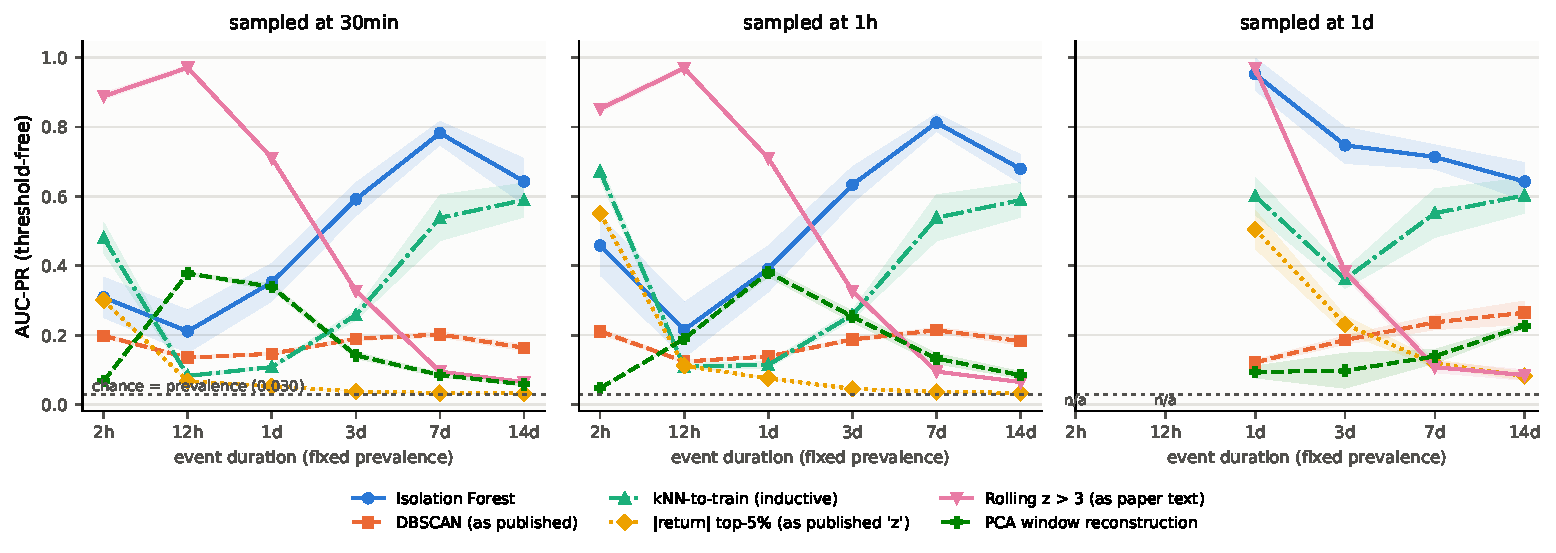
\includegraphics[width=\textwidth]{figures/fig_shift_aucpr.pdf}\\[2pt]
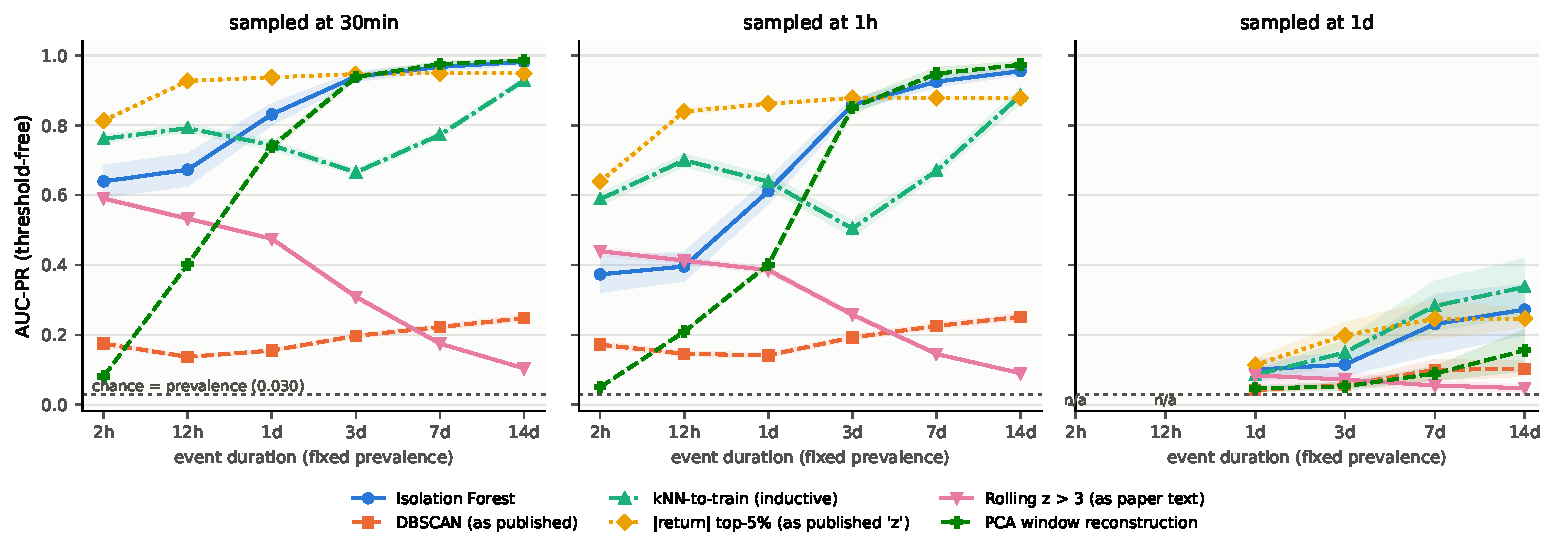
\includegraphics[width=\textwidth]{figures/fig_burst_aucpr.pdf}
\caption{Threshold-free AUC-PR versus event duration at constant prevalence (dotted line = chance $=\pi$), for level shifts (top) and variance bursts (bottom), by sampling resolution. Bands: 95\% $t$-intervals over 10 seeds.}\label{fig:aucpr}
\end{figure*}

\begin{table*}[t]
\centering\scriptsize\setlength{\tabcolsep}{4pt}
\begin{tabular}{llcllcc}
\toprule
Duration & Best (AUC-PR) & AUC-PR & 2nd best & AUC-PR & DBSCAN AUC-PR & DBSCAN alert rate \\
\midrule
2h & Rolling $z>3$ & 0.89$\pm$0.01 & kNN-to-train & 0.48$\pm$0.04 & 0.20 & 12\% \\
12h & Rolling $z>3$ & 0.97$\pm$0.01 & PCA window recon. & 0.38$\pm$0.00 & 0.14 & 21\% \\
1d & Rolling $z>3$ & 0.71$\pm$0.01 & IForest & 0.35$\pm$0.05 & 0.15 & 19\% \\
3d & IForest & 0.59$\pm$0.05 & Rolling $z>3$ & 0.33$\pm$0.01 & 0.19 & 16\% \\
7d & IForest & 0.78$\pm$0.03 & kNN-to-train & 0.54$\pm$0.07 & 0.20 & 13\% \\
14d$^\dagger$ & IForest & 0.64$\pm$0.07 & kNN-to-train & 0.59$\pm$0.05 & 0.16 & 11\% \\
\bottomrule
\end{tabular}
\\[6pt]
\begin{tabular}{llcllcc}
\toprule
Duration & Best (AUC-PR) & AUC-PR & 2nd best & AUC-PR & DBSCAN AUC-PR & DBSCAN alert rate \\
\midrule
2h & $|$return$|$ top-5\% & 0.81$\pm$0.01 & kNN-to-train & 0.76$\pm$0.01 & 0.17 & 16\% \\
12h & $|$return$|$ top-5\% & 0.93$\pm$0.00 & kNN-to-train & 0.79$\pm$0.01 & 0.14 & 21\% \\
1d & $|$return$|$ top-5\% & 0.94$\pm$0.00 & IForest & 0.83$\pm$0.03 & 0.15 & 19\% \\
3d$^\dagger$ & $|$return$|$ top-5\% & 0.95$\pm$0.00 & IForest & 0.94$\pm$0.01 & 0.20 & 15\% \\
7d$^\dagger$ & PCA window recon. & 0.98$\pm$0.01 & IForest & 0.97$\pm$0.01 & 0.22 & 13\% \\
14d$^\dagger$ & PCA window recon. & 0.99$\pm$0.01 & IForest & 0.98$\pm$0.01 & 0.25 & 12\% \\
\bottomrule
\end{tabular}

\caption{Best and second-best detector by AUC-PR at 30\,min (mean$\pm$95\% interval over 10 seeds), with DBSCAN's AUC-PR and realised alert rate. Top: level shifts; bottom: variance bursts. $^\dagger$ the two intervals overlap (a tie, not a win).}\label{tab:sweep}
\end{table*}

\paragraph{Result 1: the best detector depends on duration relative to the detector's time scale.} For level shifts (Table~\ref{tab:sweep}, top), the rolling $z$ is clearly best up to 1\,d (AUC-PR 0.89, 0.97, 0.71) consistent with its 7-day trailing baseline not yet having adapted to the shift; from 3\,d it collapses (0.33 at 3\,d, 0.10 at 7\,d), consistent with the baseline absorbing the event, and Isolation Forest is best (0.59, 0.78; a tie with kNN at 14\,d). A window-30 PCA model peaks at 12\,h--1\,d (0.38, 0.34), consistent with the event filling its 15-hour window (mechanisms here are inferred, not separately tested). For variance bursts the picture is different: a per-point $|$return$|$ rule is best up to 3\,d, and windowed or learned models catch up (statistical ties) at 7--14\,d. The ordering therefore changes with event type as well as duration, which the cross-dataset comparison could not separate.

\paragraph{Result 2: resolution alone does not reproduce the claimed DBSCAN decline.} At fixed duration, DBSCAN's F1 changes by at most 0.021 (shifts) and 0.022 (bursts) between 30\,min and 1\,h, a doubling of sample count. Against duration, DBSCAN's F1 at 30\,min is U-shaped, not monotone (shift: 0.35, 0.24, 0.26, 0.32, 0.35, 0.32 from 2\,h to 14\,d), and its AUC-PR is nearly flat (0.14--0.20). The earlier claim that DBSCAN falls monotonically with event sample count is not reproduced when prevalence, series and domain are held fixed.

\paragraph{Result 3: DBSCAN's alert rate floats, and for level shifts it dominates its F1.} DBSCAN's realised alert rate is 11--24\% for shifts and 9--21\% for bursts, against 5\% for the other detectors (Fig.~\ref{fig:alert}). Across runs, its F1 correlates $-0.92$ with that alert rate for level shifts but $+0.10$ for bursts, so the artefact is event-type dependent. Cross-dataset DBSCAN F1 values from a transductive, floating-budget detector should not be read as detection quality.

\paragraph{Result 4: thresholded F1 and AUC-PR can disagree completely.} The true rolling $z>3$ flags at most 2.0\% of points in any cell (mean over seeds), and at daily resolution its F1 is exactly 0 in every cell, while its AUC-PR is 0.97 at the 1-day event (Fig.~\ref{fig:f1}). A fixed threshold, not the score, determined the F1.

\begin{figure*}[t]
\centering
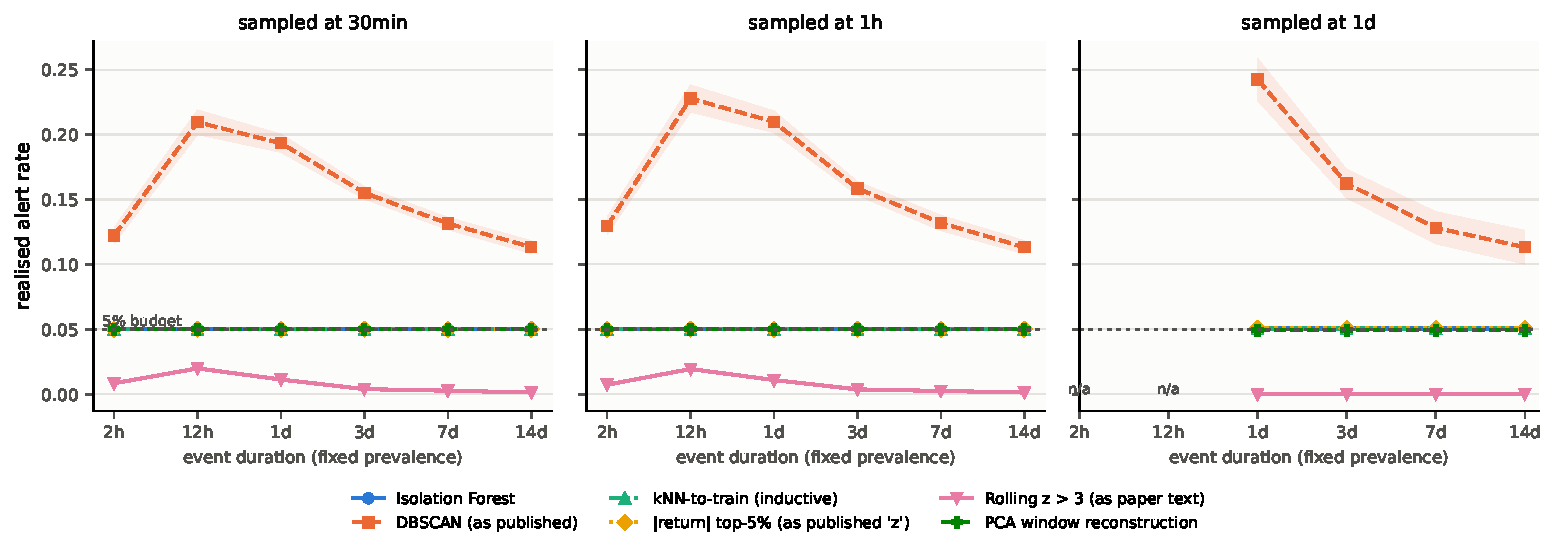
\includegraphics[width=0.92\textwidth]{figures/fig_shift_alertrate.pdf}\\[2pt]
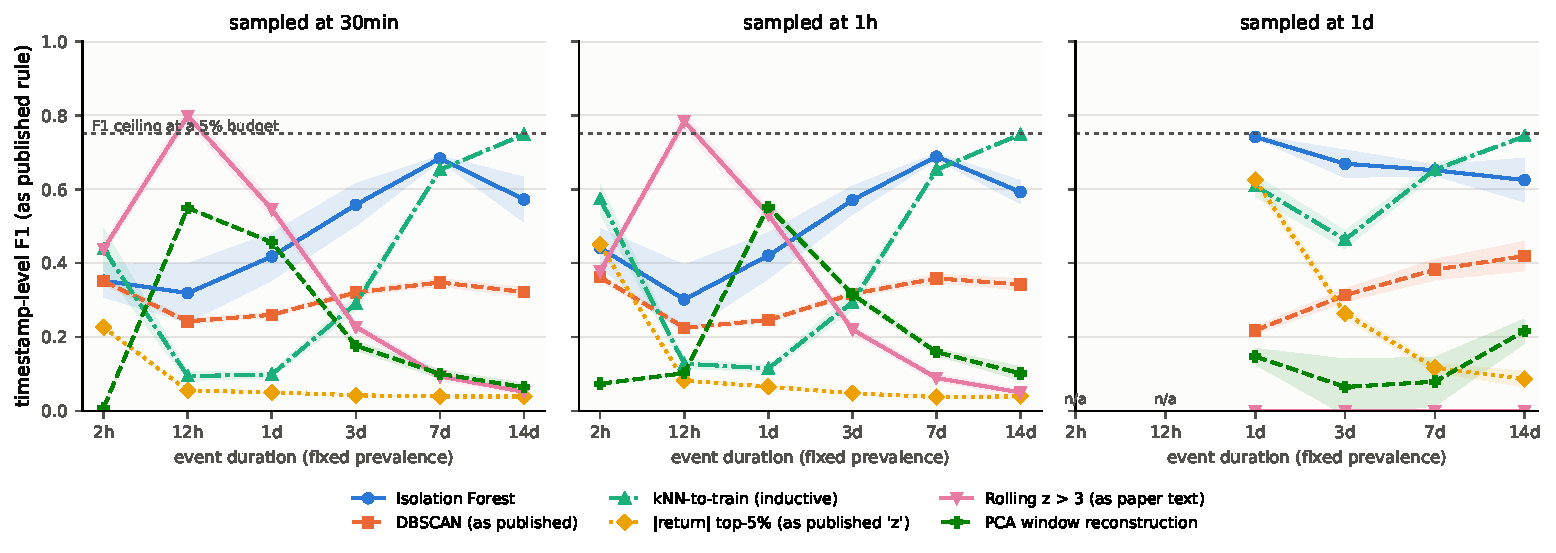
\includegraphics[width=0.92\textwidth]{figures/fig_shift_f1.pdf}
\caption{Level shifts. Top: realised alert rate; the 5\% line is the budget used by all other detectors, and DBSCAN (as published) exceeds it in every cell. Bottom: timestamp-level F1 under the published rule; the dotted line is the F1 ceiling at a 5\% budget and $\pi=3\%$ (0.75).}\label{fig:alert}\label{fig:f1}
\end{figure*}

\section{Re-evaluation of the Real-Data Results}\label{sec:real}
Table~\ref{tab:real} reports timestamp-level F1 from the stored result files, one metric throughout (LSTM = LSTM-AE, Trf. = Transformer, IF = Isolation Forest, $z$ = rolling-$z$ baseline). Study~1 uses the same-day timestamp-level table; the submitted Table~I used a hybrid of day-level precision with $\pm10$-day tolerance and event-level recall over two ``reachable'' events. These tables are from one run per dataset with seed 42 and no intervals; they are descriptive and support no ranking claim.

\begin{table}[t]
\centering\scriptsize\setlength{\tabcolsep}{1.6pt}
\begin{tabular}{llccccc}
\toprule
Data & Split & LSTM & Trf. & IF & DBSCAN & $z$ \\
\midrule
WTI & forward & \textbf{0.590} & 0.551 & 0.443 & 0.344 & 0.055 \\
Henry Hub & forward & 0.000 & 0.000 & 0.127 & \textbf{0.304} & 0.068 \\
FR Load & A & 0.060 & 0.092 & 0.029 & \textbf{0.222} & 0.055 \\
FR Load & B & 0.101 & 0.051 & 0.077 & \textbf{0.196} & 0.075 \\
FR Line Flow & B & \textbf{0.408} & \textbf{0.408} & 0.103 & 0.148 & 0.081 \\
GB demand & A & 0.000 & 0.000 & 0.000 & \textbf{0.039} & 0.019 \\
GB demand & B & \textbf{0.282} & 0.142 & 0.111 & 0.068 & 0.027 \\
ERCOT demand & A & 0.000 & 0.000 & 0.000 & \textbf{0.097} & 0.010 \\
ERCOT demand & B & 0.000 & 0.000 & 0.000 & \textbf{0.047} & 0.002 \\
\bottomrule
\end{tabular}

\caption{Timestamp-level F1 (best per row in bold); Split: forward 70/30 (A or ``forward'') or clean-window (B). Single run, seed 42.}\label{tab:real}
\end{table}

\paragraph{What changes.} On WTI the best detector under the consistent metric is the LSTM autoencoder (0.590), not DBSCAN; DBSCAN's F1 is 0.344, not the 0.695 of the hybrid metric. GB demand remains the clearest case where the LSTM leads (0.282 at the clean window). DBSCAN's F1 across datasets runs 0.344, 0.304 (daily prices), 0.222/0.196 (French load, forward/clean), 0.148 (line flow), 0.039/0.068 (GB) and 0.097/0.047 (ERCOT): lower at finer resolution overall but not monotone (ERCOT forward exceeds GB clean), and, by Sec.~\ref{sec:sweep}, confounded with event type and DBSCAN's alert rate. The selection rule and the ``detection gap'' are \textbf{withdrawn}: the gap's stated range contains GB COVID (LSTM F1 0.282 pooled over two events) and French line flow (0.408), and the rule was never tested on held-out events.

\paragraph{Per-event coverage.} Table~\ref{tab:cov} shows the fraction of each event's timestamps flagged. These come from the earlier evaluation code that excluded the final day of each event; the effect is at most one day in the event's length (1/10 for the GB cold snap, 1/70 for GB COVID) \pending{recompute with the fixed function}. On ERCOT the neural models and Isolation Forest flag none of the labelled winter events.

\begin{table}[t]
\centering\scriptsize\setlength{\tabcolsep}{3pt}
\begin{tabular}{lcccc}
\toprule
 & \multicolumn{2}{c}{GB (half-hourly)} & \multicolumn{2}{c}{ERCOT (hourly)} \\
\cmidrule(lr){2-3}\cmidrule(lr){4-5}
Detector & COVID-19 & Cold snap & Texas Freeze & Elliott \\
\midrule
LSTM-AE & 0.39 & 0.00 & 0.00 & 0.00 \\
Transformer & 0.19 & 0.00 & 0.00 & 0.00 \\
IForest & 0.15 & 0.00 & 0.00 & 0.00 \\
DBSCAN & 0.09 & 0.09 & 0.07 & 0.26 \\
Rolling $z$ & 0.03 & 0.05 & 0.01 & 0.00 \\
\bottomrule
\end{tabular}

\caption{Per-event coverage (fraction of event timestamps flagged), clean-window protocol, pre-fix evaluation code.}\label{tab:cov}
\end{table}

\section{Discussion: a Checklist}
The sweep suggests reporting, for any energy anomaly benchmark: (1) event-level and timestamp-level metrics separately; (2) prevalence, realised alert rate and $\F^{\max}$; (3) a threshold-free metric alongside any fixed-threshold F1; (4) inductive fitting, or explicit disclosure of transductive fits; (5) constant prevalence when varying event duration, and independent variation of resolution and duration; (6) per-event results and no ranking from one or two events; (7) tiered labels with the tier that was fixed \emph{before} modelling kept separate from post-hoc ones.

\section{Limitations}\label{sec:limits}
\begin{itemize}
\item The sweep is synthetic, uses one magnitude (3 s.d.), two event types, a hand-built generator, and a PCA surrogate instead of neural detectors; conclusions about the real grid are not implied. \pending{neural models in the sweep; additional magnitudes}
\item Real-data tables are single runs with one or two events per dataset, no intervals and no repeated training. \pending{block bootstrap, repeated seeds, rolling-origin splits; additional documented events}
\item Hyperparameters in the real-data tables are fixed defaults. An earlier CMA-ES search used test-set F1 as its objective and shorter training than the study scripts, so it must not be cited as validated tuning. Equal-budget tuning on a synthetic validation split, with real test events untouched, is implemented but not yet run on real data. \pending{run equal\_budget\_tuning.py on GB and ERCOT; neural families on GPU}
\item Resolution ablation on the \emph{real} series (same events, resampled) is implemented but not yet run. \pending{run real\_resolution\_ablation.py}
\item The sequence models in Studies 2--4 build windows across the gap in the clean-window test set (about 30 windows) and scores are index-aligned by an implicit offset; the new windowing code removes both issues but published neural numbers were not regenerated. \pending{re-run neural models with segment-aware windows}
\item Event windows are curated; stronger recent detectors and VUS-PR are not evaluated.
\end{itemize}

\section{Conclusion}
Under one evaluation contract, the earlier duration--resolution selection rule and detection gap do not survive, and the figures that appeared to support them traced to mixed metrics, floating alert budgets and uncontrolled variables. In a constant-prevalence sweep the best detector depends on how an event's duration compares with a detector's own time scale and on the event type, and resolution alone has little effect on DBSCAN. The value of the work is the evaluation contract, the controlled design and the released tests, not a new selection rule.

\section*{Reproducibility}
Code, tests (including regression tests for the event-end-day and window-seam bugs), result files and this paper's table generator are at \url{https://github.com/suyounas/energy-anomaly-benchmark-4d}; commit \texttt{\textless COMMIT-HASH\textgreater}, archived DOI \texttt{\textless ZENODO-DOI\textgreater}. \pending{fill commit hash and Zenodo DOI after the final push} All quoted numbers are generated by \texttt{paper/revised/make\_tables.py} from CSVs.

\section*{Acknowledgment}
The author thanks Andrew Howe for a published account of applied anomaly-detection work in commodity analytics that motivated the framing. (A statement in the earlier version that an ATLAS statistical framework was ``adapted'' has been removed because no such adaptation is described.)

\begin{thebibliography}{99}\small
\bibitem{kim2022rigorous} S.~Kim, K.~Choi, H.-S.~Choi, B.~Lee, S.~Yoon, ``Towards a rigorous evaluation of time-series anomaly detection,'' in \emph{Proc.\ AAAI}, vol.~36, no.~7, pp.~7194--7201, 2022.
\bibitem{wu2023flawed} R.~Wu and E.~J.~Keogh, ``Current time series anomaly detection benchmarks are flawed and are creating the illusion of progress,'' \emph{IEEE Trans.\ Knowl.\ Data Eng.}, vol.~35, no.~3, pp.~2421--2429, 2023.
\bibitem{schmidl2022comprehensive} S.~Schmidl, P.~Wenig, T.~Papenbrock, ``Anomaly detection in time series: a comprehensive evaluation,'' \emph{PVLDB}, vol.~15, no.~9, pp.~1779--1797, 2022.
\bibitem{wenig2022timeeval} P.~Wenig, S.~Schmidl, T.~Papenbrock, ``TimeEval: a benchmarking toolkit for time series anomaly detection algorithms,'' \emph{PVLDB}, vol.~15, no.~12, pp.~3678--3681, 2022.
\bibitem{paparrizos2022tsb} J.~Paparrizos, Y.~Kang, P.~Boniol, R.~S.~Tsay, T.~Palpanas, M.~J.~Franklin, ``TSB-UAD: an end-to-end benchmark suite for univariate time-series anomaly detection,'' \emph{PVLDB}, vol.~15, no.~8, pp.~1697--1711, 2022.
\bibitem{paparrizos2022vus} J.~Paparrizos, P.~Boniol, T.~Palpanas, R.~S.~Tsay, A.~Elmore, M.~J.~Franklin, ``Volume under the surface: a new accuracy evaluation measure for time-series anomaly detection,'' \emph{PVLDB}, vol.~15, no.~11, pp.~2774--2787, 2022.
\bibitem{liu2024elephant} Q.~Liu and J.~Paparrizos, ``The elephant in the room: towards a reliable time-series anomaly detection benchmark,'' in \emph{NeurIPS Datasets and Benchmarks Track}, 2024.
\bibitem{darban2024survey} Z.~Z.~Darban, G.~I.~Webb, S.~Pan, C.~C.~Aggarwal, M.~Salehi, ``Deep learning for time series anomaly detection: a survey,'' \emph{ACM Comput.\ Surv.}, 2024, doi:10.1145/3691338.
\bibitem{gillioz2025dataset} M.~Gillioz, G.~Dubuis, P.~Jacquod, ``A large synthetic dataset for machine learning applications in power transmission grids,'' \emph{Scientific Data}, vol.~12, p.~168, 2025.
\bibitem{ercot2023records} ERCOT, ``2023 peak demand records,'' \url{https://www.ercot.com/static-assets/data/news/content/a-peak-demand/2023/all-time-records.htm} (records are unofficial until final settlement).
\bibitem{liu2008iforest} F.~T.~Liu, K.~M.~Ting, Z.-H.~Zhou, ``Isolation forest,'' in \emph{Proc.\ IEEE ICDM}, pp.~413--422, 2008.
\bibitem{hochreiter1997lstm} S.~Hochreiter and J.~Schmidhuber, ``Long short-term memory,'' \emph{Neural Computation}, vol.~9, no.~8, pp.~1735--1780, 1997.
\bibitem{vaswani2017attention} A.~Vaswani et al., ``Attention is all you need,'' in \emph{Adv.\ Neural Inf.\ Process.\ Syst.}, vol.~30, 2017.
\bibitem{ester1996dbscan} M.~Ester, H.-P.~Kriegel, J.~Sander, X.~Xu, ``A density-based algorithm for discovering clusters in large spatial databases with noise,'' in \emph{Proc.\ ACM SIGKDD}, pp.~226--231, 1996.
\end{thebibliography}
\end{document}
